\documentclass[11pt]{article}
\usepackage{float}
\parindent 0px
\usepackage[utf8]{inputenc}
\usepackage{biblatex}
\addbibresource{ref.bib}
\usepackage{color}
\usepackage{xcolor}
\usepackage{graphicx}
\usepackage{multicol}
\usepackage{multirow}
\usepackage[T1]{fontenc}
\usepackage{enumerate}
\usepackage{float}
\usepackage{amsmath,mathtools,amssymb,amsfonts}
\usepackage{physics}
\usepackage{hyperref}
\usepackage[margin=1in]{geometry}
\title{CSE 300: Online Assignment}
\author{Md Shamsuzzoha Bayzid, Mahjabin Nahar, Md Shariful Islam Bhuyan,
and Md Saidur Rahman}
\date{April, 2021}
\begin{document}
\maketitle
\section{Introduction}
This assignment has been designed to assess the preparation of the students in writing
scientific articles using \LaTeX. This assignment covers a variety of components that are
commonly used in scientific manuscripts.
\subsection{Figure}
We intend to put Figure 1 at the top of a page.
\begin{figure}[t]
	\centering
	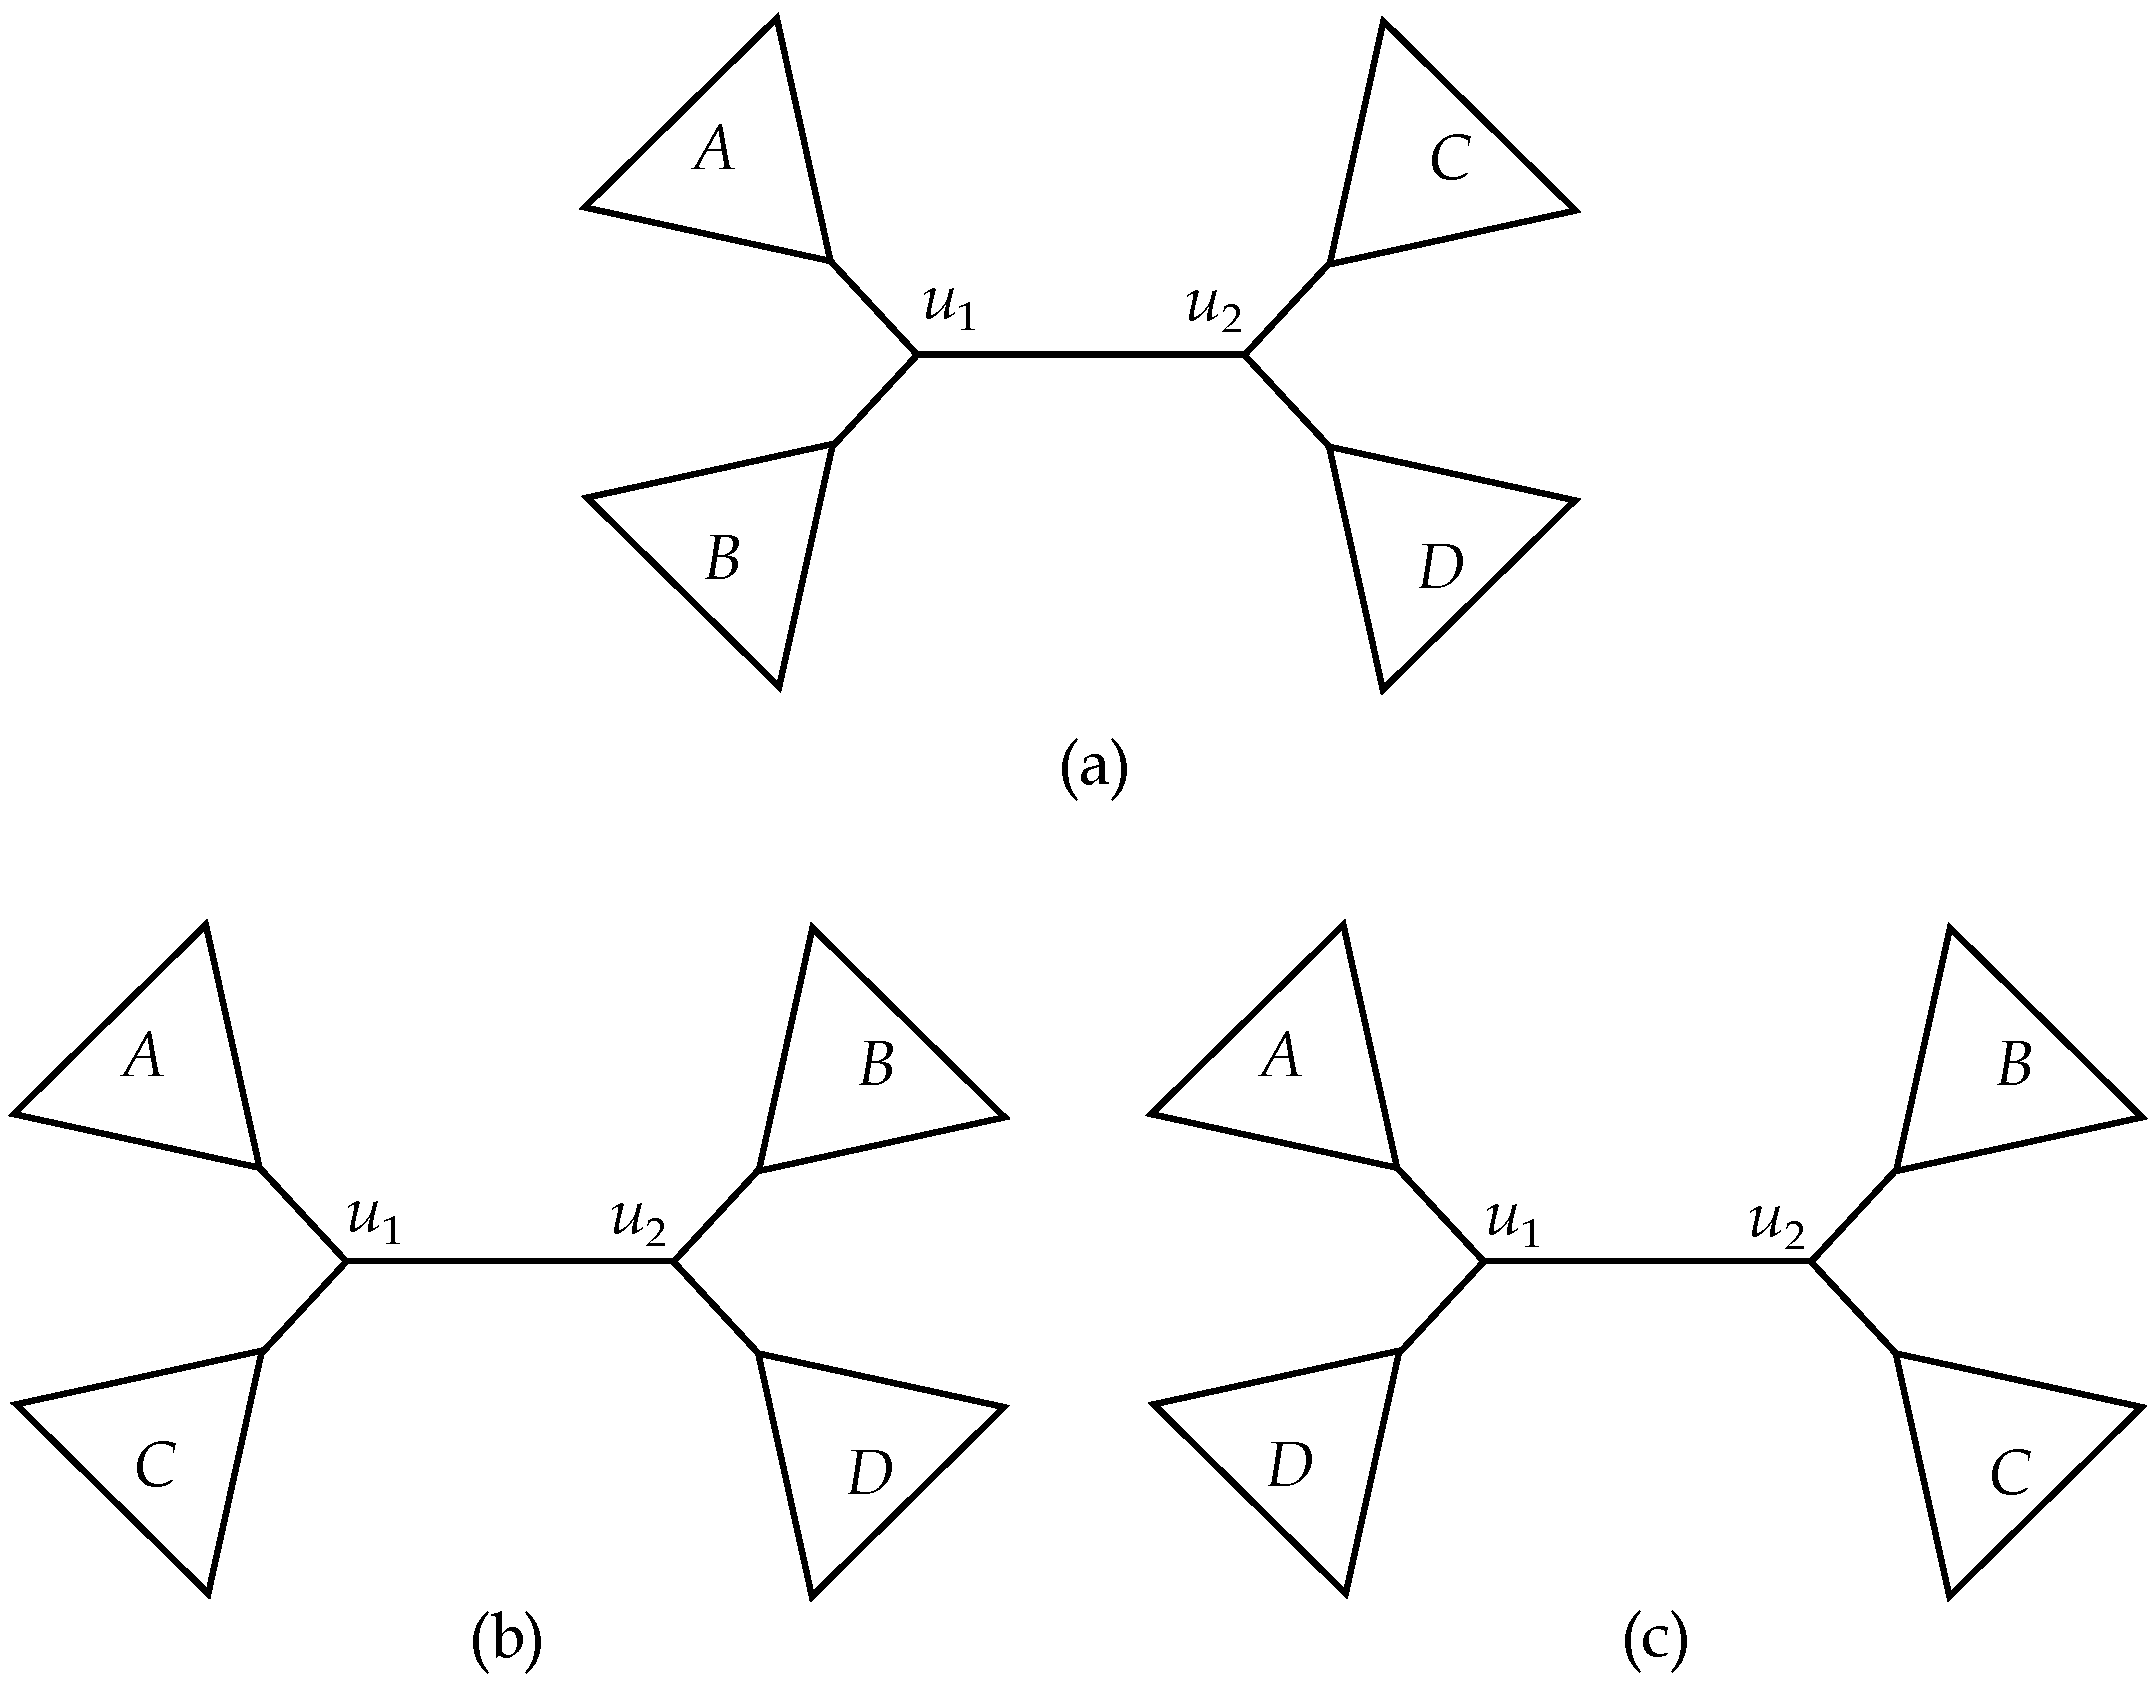
\includegraphics[width=5cm,height=5cm,scale=0.4]{17-CSE300_online-Figure3.pdf}
	\caption{\textbf{Nearest Neighbor Interchange (NNI) move on an internal edge.} (a) A species tree ST, and (b)-(c) the neighbors of ST resulting from one NNI move on edge e = (u1, u2). A, B, C, and D are the sets of taxa in the four subtrees around edge e.}
\end{figure}
\subsection{Tables}
We wish to place Table 1 right here.
\begin{table}[H]
    \centering
    \caption{ \textbf{Optimization scores for Method-1 and Method-2 on different datasets covering various model conditions.} We show average scores of two optimization criteria for various model conditions.}
    \vspace{1cm}
    \begin{tabular}{|c c|c c|c c|}
       \hline
       Dataset & Model & \multicolumn{2}{|c|}{Optimization Score 1} & \multicolumn{2}{|c|}{Optimization Score 2} \\
      \cline{3-6}
       & condition & Method-1 & Method-2 & Method-1 & Method-2\\
      \hline
     \hline
     \multirow{4}{*}{D1} & M1 & 7,425.55  & 770.00 & 929.55 & 10\\
     & M2 & 7,657.00 & 9,179.00 & 716.15 & 20\\
     & M3 & 54.00 & 9,007.15 & 3,759.00 & 30 \\
     & M4 & 74.00 & 5567.15 & 99.00 & 25 \\
      \hline
     \multirow{3}{*}{D2} & M1 & 34.00 & 273.00 & 321.60 & 34\\
     & M2 & 357.00 & 79.60 & 16.00 & 11\\
     & M3 &  657.00 & 179.60 & 716.00 & 19\\
      \hline
    \end{tabular}
\end{table}
\pagebreak
\subsection{Equations}
Let n1|n2|n3 be a tripartition defined on an internal node u of a binary tree T. The number of tripartitions mapped to u is given by Eqn. 1.
\begin{equation}
   \mathcal{N Q} (n1,n2,n3)= \binom{n1}{2} \binom{n2}{1} \binom{n3}{1} + \binom{n2}{2} \binom{n1}{1} \binom{n3}{1}
   + \binom{n3}{2} \binom{n1}{1} \binom{n2}{1}
   \end{equation}
 \section{Conclusions}
 The major objectives of this assignment are listed below (please do not ignore the font sizes).
 \begin{enumerate}
     \item \begin{Large} To assess the ability of the students in preparing manuscripts in  \LaTeX. \end{Large}
     \item \begin{large} To see if the students have adequately practiced different aspects of writing in  \LaTeX . \end{large}
     \item \begin{normalsize} To see if the students can add various basic components (e.g., tables, figures, equations) to a 
     \LaTeX \space manuscript. \end{normalsize}
     \pagebreak
      \item \begin{scriptsize} To see if the students can leverage the available materials (both offline and online) to do something which has not explicitly been taught in the class. \end{scriptsize}
 \end{enumerate}
\printbibliography
\end{document}